\documentclass[10pt, twocolumn]{article}

\usepackage[export]{adjustbox}
\usepackage{algorithm}
\usepackage[noend]{algpseudocode}
\usepackage{amsfonts}
\usepackage{amsmath}
\usepackage{amssymb}
\usepackage{amsthm}
\usepackage{bm}
\usepackage{booktabs}
\usepackage{caption}
\usepackage{float}
\usepackage[a4paper, margin=1in]{geometry}
\usepackage{graphicx}
\usepackage{hyperref}
\usepackage{lipsum}
\usepackage{mathrsfs}
\usepackage{mleftright}
\usepackage[round]{natbib}
\usepackage{parskip}
\usepackage{physics}
\usepackage{subcaption}
\usepackage{tabularx}
\usepackage{times}

\setlength\columnsep{0.6cm}
\setlength{\fboxrule}{0.5pt}
\setlength{\fboxsep}{0pt}

\theoremstyle{definition}
\newtheorem{definition}{Definition}
\newtheorem{notation}{Notation}
\newtheorem{theorem}{Theorem}
\theoremstyle{remark}
\newtheorem{remark}{Remark}

\makeatletter
\newcommand\outauthor{%
	\begin{tabular}[t]{c}
		\@author
	\end{tabular}
}
\renewcommand\maketitle{%
	\par
	\twocolumn[{%
		\centering
		{\Large\bfseries\@title\par}
		\vskip 0.2in plus 1fil minus 0.1in
		{\large\outauthor\par}
		\vskip 0.3in plus 2fil minus 0.1in
	}]%
}
\makeatother

\makeatletter
\def\thm@space@setup{\thm@preskip=\parskip\thm@postskip=0pt}
\makeatother

\newcommand{\E}{\mathbb{E}}
\newcommand{\N}{\mathbb{N}}
\newcommand{\R}{\mathbb{R}}
\newcommand{\Z}{\mathbb{Z}}

\title{Snekboros: Vision World Models for Snake Playing}
\author{\small
    1006652 Lee Jun Hui Ryan, 1006895 Wang Yihe,
    1007036 Celest Teng Roh Yee, 1007485 Gregory Lim Eu Rhen
}
\date{April 2026}

\begin{document}

\maketitle

\section{Introduction}

Arguably, AI systems today do not possess ``human-level intelligence'' for many important real-world tasks.
Driving is a common example:
humans can learn the basics in days,
yet level-five autonomous driving remains out of reach
even with millions of hours of data.
World models have been proposed
as a promising approach to human-level AI.
Broadly,
a world model learns a representation of its environment,
and how to evolve that representation through action,
thus ``learning the consequences of their actions''.
To reach a particular goal at inference,
a world model can be used to plan action sequences
optimising a particular objective.
In recent years, world models have demonstrated promise in learning tasks
ranging from robotic manipulation to video game playing on relatively low sample counts.
For this reason, we believe world models present an exciting opportunity for innovation in AI.

\begin{center}
    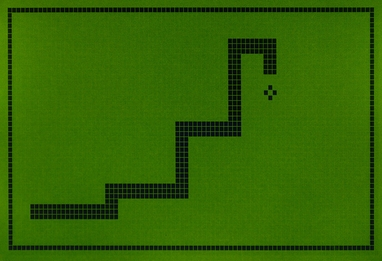
\includegraphics[width=0.4\linewidth]{images/snake.jpg}
    \captionof{figure}{Snake on a Nokia 6110 phone.}
\end{center}

Snake is a classic action video game where the player controls the end of a growing line segment on a planar region, steering it left, right, up, and down to consume food without colliding with walls or snake segments \citep{wikipedia2026snake1998}.
Although Snake has simple rules,
games often require long-horizon planning,
as a single wrong move early on can be fatal.
In 2018, OpenAI released a set of research requests, one of which asked researchers to train a machine learning model to beat the classic Snake game.
This request serves as the impetus for our research project \citep{openai2018requests}.\footnote{We believe Snake to be an unusually clean testbed for world modelling as it admits a trivial solution---moving along a Hamiltonian cycle---on grids with even dimension.}

In this paper, we investigate the use of vision world models---world models with visual input---for the game of Snake.
Our contributions are threefold.
First, we formulate Snake as a vision-based problem.
Second, we train and test world models for Snake playing.
Third, we compare and interpret the pros and cons of various approaches.
Our code repository can be found at \href{https://github.com/gregorylimeurhen/snekboros}{github.com/gregorylimeurhen/snekboros}.
Snekboros aims to contribute most directly to SDG 9 (Industry, Innovation, and Infrastructure) by advancing world model research.

\section{Existing Work}

Model-based learning, an approach in which
an agent learns an internal model of environment dynamics,
has a long history in robotics \citep{sutton1991dyna, holkar2011mpc, williams2017mppi}.
By learning to predict how an environment evolves,
world models enable agents to reason about possible futures, in a process analogous to human imagination.

Generative world models learn to predict environment dynamics in pixel space, acting as learned simulators that generate future observations from a history of past states and actions.
Historically, these models have been fairly successful in various games \citep{hafner2025dreamerv4, micheli2023iris, decart2024oasis, alonso2024diamond}.
However, these models predict in high-dimensional pixel space, which can be computationally expensive \citep{ko2023actionless}.
Additionally, these models risk wasting capacity on learning task-irrelevant noise as details in pixel space are not always predictable.
These models also sometimes use task-specific state-based objectives, which hinder adaptation to new tasks.

The Joint Embedding Predictive Architecture (JEPA) has emerged as a promising way for world models to learn to predict environment dynamics in representation space \citep{lecun2022autonomous}.
JEPA has prominently been applied
for self-supervised representation learning
by predicting masked image patches in representation space \citep{assran2023ijepa, bardes2024vjepa, assran2025vjepa2}.
However, JEPA admits a trivial solution
that leads to representation collapse,
as the encoder can learn to map all observations
to a single representation.
Early approaches tried to address this collapse
by devising a gradient-free ``target encoder''
that tracks an exponential moving average
of the (actual) encoder.
Other approaches, such as DINO-WM,
simply use frozen pretrained vision encoders \citep{zhou2025dinowm}.
Although this prevents representation collapse
and can make training more straightforward,
this could closely tie a system to its encoder's input resolution,
and relies on how well the pretrained weights match the (actual) task.

Model predictive control (MPC) predicts and evaluates candidate action sequences online, and has demonstrated its ability to ground real-time dynamical models at the cost of increased computation.
However, many works only focus on standard robotics tasks
with explicit goal states (e.g. Maze, Wall, PushT, Reach, etc.) used as input at test time. \citep{fu2021d4rl, tassa2018dmcontrol}.
Our work explores MPC-style approaches that have no such input at test time.

\section{Methodology}

\subsection{Data}

Let $L\in 2\N_{\geq 1}$ be a grid extent,
and $U\in\N_{\geq 1}$ be an upsampling factor,
and $D\in\N_{\geq 1}$ be a time horizon,
and $\mathcal{G}=[L]^{2}$ be a grid,
and $\preceq$ be the row major order of $\mathcal{G}$,
and $\mathcal{X}=[0,1]^{LU\times LU\times 3}$ be an image space.

\begin{definition}[Action Space]
$$
	\mathcal{A}
    =
    \mleft\{-1,0,1\mright\}
$$
\end{definition}

\begin{definition}[Movement Space]
$$
	\mathcal{M}
	=
	\mleft\{(0,1),(0,-1),(-1,0),(1,0)\mright\}
$$
\end{definition}

\begin{definition}[Rotation Function]
\begin{align*}
	R&:\Z^{2}\to\Z^{2}
	\\
	R\mleft(x,y\mright)
    &=
    \mleft(y,-x\mright)
\end{align*}
\end{definition}

The action space contains actions for ``left'', ``right'', and ``straight''.
The movement space contains movements for ``up'', ``down'', ``left'', and ``right''.
The rotation function rotates a grid position clockwise by 90$^{\circ}$.

\begin{algorithm}[H]
\caption{$\textsc{Simulate}(\delta)$}
\begin{algorithmic}
	\Require $\delta:\N\to\mathcal{A}$
	\State ${
		\bm{s}
		\sim
		\mathcal{U}(
			\{
				\bm{s}
				:
				[2]
				\to
				\mathcal{G}
				\mid
				s_{2}-s_{1}
				\in
				\mathcal{M}
			\}
		)
	}$
	\State ${
		E
		\gets
		\mathcal{G}
		\setminus
		\{
			s_{i}
			\mid
			i\in[\abs{\bm{s}}]
		\}
	}$
	\State $f\gets\min_{\preceq}E$

	\State $t\gets 0$
	\While{$\bm{s}\neq\mathord{\perp}$}
		\State $i_{f}\gets 0$
		\State $a\gets\delta(t)$
		\State $h\gets s_{1}+R^{a}(s_{1}-s_{2})$
		\If{$h=f$}
			\State ${
				\bm{s}
				\gets
				h
				\parallel
				(s_{i})_{i=1}^{\abs{\bm{s}}}
			}$
			\State $i_{f}\gets 1$
		\Else{}
			\State ${
				\bm{s}
				\gets
				h
				\parallel
				(s_{i})_{i=1}^{\abs{\bm{s}}-1}
			}$
		\EndIf

		\State ${
			B
			\gets
			\{
				s_{i}
				\mid
				i\in[2..\abs{\bm{s}}]
			\}
		}$

		\If{$s_{1}\notin\mathcal{G}\setminus B$}
			\State $\bm{s}\gets\mathord{\perp}$
		\EndIf

		\If{$\bm{s}\neq\mathord{\perp}\land i_{f}=1$}
			\State ${
				E
				\gets
				\mathcal{G}
				\setminus
				\mleft\{
					s_{i}
					\mid
					i\in[\abs{\bm{s}}]
				\mright\}
			}$
			\If{$E=\varnothing$}
				\State $f\gets\mathord{\perp}$
			\Else{}
				\State $f\gets\min_{\preceq}E$
			\EndIf
		\EndIf

		\State $t\gets t+1$
	\EndWhile
\end{algorithmic}
\end{algorithm}

% Rules
The game starts by spawning a length-$2$ snake in random adjacent cells.
At each tick, the snake takes an action to move its segments,
and the food spawns in the first cell under row-major order if there is an unoccupied cell and every cell is unoccupied by food.
The snake dies if its first segment moves out of the grid or into a cell occupied by another segment.
The snake grows by $1$ (from its last segment) if its first segment moves into a cell occupied by food.
The snake wins if its segments cover the grid.

For experimental reproducibility, we use a fixed, global seed for each pseudorandomly generated quantity.
We set $L=4$ and $U=1$ to keep computation tractable
while keeping planning non-trivial.

% Policy
To avoid manually playing the game,
we generate episodes using a perturbed Hamiltonian policy
with first-action off-policy branching on each game tick for coverage of a large and diverse number of plausible game states \citep{tapsell2015snake}.
For each trajectory, we store label
$$
(\mathfrak{S},(\mathfrak{C}_{t})_{t=1}^{D})
$$
where survival label $\mathfrak{S}$ is $1$
if the snake survived the trajectory (and $0$ otherwise),
and for each $t\in[D]$, consumption label $\mathfrak{C}_{t}$ is $1$
if the snake consumed at game tick $t$ (and $0$ otherwise).

Each unoccupied cell is coloured black.
Each cell occupied by a snake segment $s_{i}\in\bm{s}$ is coloured blue with brightness $1-(i-1)/L^{2}$
for each $i\in[\abs{\bm{s}}]$.
Each cell occupied by food is coloured green.
When the snake dies (resp. wins), each cell becomes and remains black (resp. white) for the remainder of the trajectory.
The cells are coloured in this non-overlapping way to ensure injectivity for the game to be Markovian after snake spawning.
The grid is rendered at arbitrary scale by rasterisation.

For each starting position, we generate $1$ episode,
and the data is split by episode into training, validation, and testing sets in a ratio of $8$-$1$-$1$.

\subsection{Architecture}

Let $\mathcal{H}\in\{\R^{H}\mid H\in\N_{\geq 1}\}$ be a hidden space,
and $\tau\in[0,1]$ be a survival threshold,
and $\bm{\gamma}\in[0,1]^{D}$ be a discount.

\begin{definition}[Encoder]
$$
	\phi:\mathcal{X}\to\mathcal{H}
$$
\end{definition}

\begin{definition}[World Model]
\begin{align*}
	\mathscr{F}
	&:
	\mathcal{H}\times\mathcal{A}
	\to
	\mathcal{H}
\end{align*}
\end{definition}

\begin{definition}[Evaluator]
\begin{align*}
	% "split into heads, then merge into a sum with coefficient"
	\mathscr{V}_{S}
	&:
	\mathcal{H}^{D} % trajectory
	\to
	[0,1] % probability of surviving within horizon
	\\
	\mathscr{V}_{C}
	&:
	\mathcal{H}^{D} % trajectory
	\to
	[0,1]^{D} % probability of consumption at state, for each state of trajectory
	\\
	\mathscr{V}
	&:
	\mathcal{H}^{D} % trajectory
	\to
	\R_{\geq 0}
	\\
	\mathscr{V}(\bm{h})
	&=
	\mathbf{1}_{
		\mathscr{V}_{S}(\bm{h})
		\geq
		\tau
	}
	\bm{\gamma}^{\top}
	\mathscr{V}_{C}(\bm{h})
\end{align*}
\end{definition}

\begin{figure}[H]
	\centering
	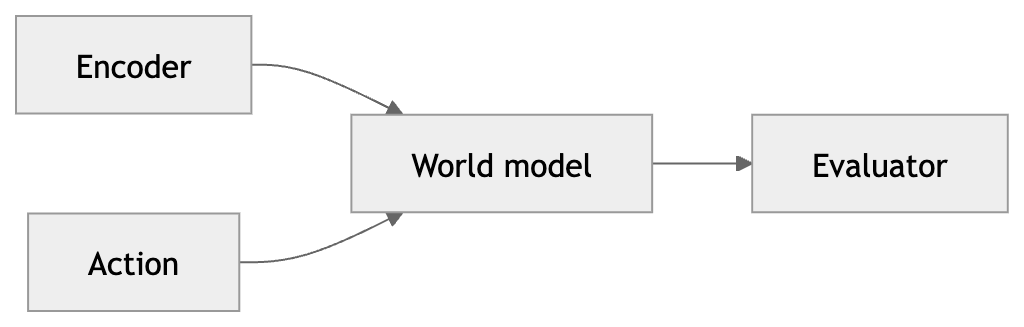
\includegraphics[width=0.9\linewidth]{images/architecture.png}
\end{figure}

The system consists of three components:
an encoder, a world model, and an evaluator.
The encoder maps
an image $x\in\mathcal{X}$
into a representation $h\in\mathcal{H}$
that aims to capture abstract information needed for effective downstream prediction by eliminating unnecessary detail.
The world model, conditioned on
an action $a\in\mathcal{A}$, maps
a representation $h\in\mathcal{H}$ to
a next representation $h'\in\mathcal{H}$
that aims to represent the state of the game
at the next game tick.
The evaluator maps
a representation sequence $\bm{h}\in\mathcal{H}^{D}$ to
a number $r\in\R_{\geq 0}$
that aims to measure how good (or bad) the state corresponding to that representation is.
The evaluator has a survival head and a consumption head.
The survival (resp. consumption) head learns to predict the probability of (i.e. approximate the) survival (resp. consumption) labels.

Our components use
convolutional and gated recurrent unit (GRU)
architectures.
Our encoder uses a convolutional architecture,
while our world model and evaluator use convolutional GRU architectures.

% Optimiser and loss
We use both one-step teacher-forced
and multi-step free-running loss terms
to supervise individual transitions
and enforce consistency on rollouts.
The world model uses mean squared error (MSE) loss with stop gradients on encoded successors.
The evaluator uses binary cross-entropy (BCE) loss on survival and consumption labels.

There is a trivial solution where the encoder maps all observations to a single representation.
To avoid this ``representation collapse'', we apply sketched isotropic Gaussian regularisation (SIGReg) for representations to follow an approximately isotropic Gaussian distribution \citep{balestriero2025lejepa}.
We monitor training for representation collapse by tracking the effective rank of the centred and flattened representations.

We train the system in phases for numerical stability.
The first $20\%$ of epochs only update encoder weights.
The next $20\%$ of epochs only update world model weights.
The last $60\%$ of epochs update encoder, world model, and evaluator weights.

% In essence, we have:
% \lambda_\mathrm{encoder}\mathcal{L}_\mathrm{encoder}
% + \lambda_\mathrm{wm}\mathcal{L}_\mathrm{wm}
% + \lambda_\mathrm{evaluator}\mathcal{L}_\mathrm{evaluator}

Inference returns the first element of
$$
	\arg\max_{\bm{a}\in\mathcal{A}_{\checkmark}^{D}(x)}
	\mathscr{V}\mleft(
		\mleft[
			\mleft(
				\bigcirc_{i=1}^{t}
				\mathscr{F}_{a_{i}}
			\mright)
			\mleft(
				\phi(x)
			\mright)
		\mright]_{t=1}^{D}
	\mright)
$$
where $x\in\mathcal{X}$ is an image,
and $\mathcal{A}_{\checkmark}^{D}(x)\subseteq\mathcal{A}^{D}$ is the space of legal length-$D$ action sequences from the game state implied by $x$.
As enumerating over all action sequences is often intractable,
we sample using a (first-action-)stratified random method.
We set the action sequence sample count to $1024$ to balance
computational tractability with planning quality.
Ties are broken randomly over first actions of optimal legal sequences.
We set $\tau=0.25$ to balance snake aggression with conservativeness.
We set $D=L^{2}-1$ as it is the maximum length of a simple path on $\mathcal{G}$.
We set $\bm{\gamma}=((1-1/D)^{t-1})_{t=1}^{D}$ for food consumption to matter more earlier.

\section{Experimentation}

In a game, a snake can consume a maximum of $L^{2}-2$ foods (in total).
Thus, we define the completion rate of a game as the fraction of foods consumed by a snake in that game.
We make completion rate our scoring metric
since in a game, a snake wins by consuming the maximum number of foods.
To prevent a snake from prolonging a game indefinitely by looping, we enforce a maximum of $1000$ game ticks, beyond which the snake is considered dead.

% ablate: survival_threshold = 0.25 (def), 0.5, 0.0
% ablate: planner_depth = 15 (def), 10, 5
% ablate: planner_samples = 1024 (def), 512, 2048

\begin{center}
\begin{tabular}{ll}
\toprule
\textbf{Survival threshold} & \textbf{Score} \\
\midrule
0.00 & 0.86 \\
0.25 (baseline) & 0.89 \\
0.50 & 0.86 \\
\bottomrule
\end{tabular}
\captionof{table}{Effect of survival threshold on score.}
\end{center}

We ablated the survival threshold
over $\{0.00, 0.25, 0.50\}$.
The intermediate threshold achieved the highest score, suggesting that a mild survival constraint improves planning without being overly restrictive.

\begin{center}
\begin{tabular}{ll}
\toprule
\textbf{Time horizon} & \textbf{Score} \\
\midrule
5 & 0.14 \\
10 & 0.75 \\
15 (baseline) & 0.89 \\
\bottomrule
\end{tabular}
\captionof{table}{Effect of time horizon on score.}
\end{center}

We ablated the time horizon
over $\{5, 10, 15\}$.
Performance decreased
slightly from $15$ to $10$,
and sharply from $10$ to $5$,
suggesting that the task benefits from longer-horizon planning.

\begin{center}
\begin{tabular}{ll}
\toprule
\textbf{Sampling method} & \textbf{Score} \\
\midrule
Random & 0.89 \\
Stratified random (baseline) & 0.89 \\
Cross-entropy & 0.86 \\
\bottomrule
\end{tabular}
\captionof{table}{Effect of sampling method on score.}
\end{center}

We ablated the action sequence sampling methods
over random, stratified random, and cross-entropy methods \citep{rubinstein1999crossentropy}.
Performance was similar across methods, suggesting that the choice of sampling method was not a major performance factor.

\begin{center}
\begin{tabular}{ll}
\toprule
\textbf{Sample count} & \textbf{Score} \\
\midrule
512 & 0.79 \\
1024 (baseline) & 0.89 \\
2048 & 0.93 \\
\bottomrule
\end{tabular}
\captionof{table}{Effect of sample count on score.}
\end{center}

We ablated the action sequence sample count
over $\{512, 1024, 2048\}$.
Performance improved from $512$ to $1024$,
with diminishing returns at $2048$,
suggesting that $1024$ samples were fairly sufficient for effective planning on our task.

\begin{center}
\begin{tabular}{ll}
\toprule
\textbf{Architecture} & \textbf{Score} \\
\midrule
Ours (baseline) & 0.89 \\
DINO-WM & 0.00 \\
\bottomrule
\end{tabular}
\captionof{table}{Effect of architecture on score.}
\end{center}

We tested our system architecture against
one that borrows elements from DINO-WM \citep{zhou2025dinowm}.
The latter uses a DINOv2 ViT-S/14 architecture for the encoder,
and a transformer architecture for the world model \citep{oquab2023dinov2}.
The DINO-WM architecture failed to complete the task.
Because the encoder weights were frozen after ImageNet pre-training, we hypothesise that this failure can be attributed to limited task adaptation and the larger architecture requiring more data than was available.

\begin{figure}[htbp]
	\centering
	
\includegraphics[width=0.23\textwidth, frame]{images/win/0690.png}
	
\includegraphics[width=0.23\textwidth, frame]{images/win/0691.png}
	
\includegraphics[width=0.23\textwidth, frame]{images/win/0692.png}
	
\includegraphics[width=0.23\textwidth, frame]{images/win/0693.png}
	\caption{Snake win.}
\end{figure}

The snake was able to win when we sampled using the random method with $\tau=0$.
We hypothesise that this was because the final foods often require aggressive, nearly terminal manoeuvres.
At high snake lengths, the legal path to the last food may simply pass through states that the survival head assigns low probability to,
because such states are rare in the training data,
or because small prediction errors are amplified when the board is almost full.
When $\tau>0$, the planner may thus discard these risky-looking trajectories in favour of safer actions that prolong the game without completing it.

\begin{center}
\begin{tabular}{ll}
\toprule
\textbf{System} & \textbf{Score} \\
\midrule
Random policy & 0.00 \\
Ours & 0.89 \\
Oracle planner & 1.00 \\
Hamiltonian cycle policy & 1.00 \\
\bottomrule
\end{tabular}
\captionof{table}{Comparison of systems by score.}
\end{center}

We compared our system against
a random policy,
an oracle planner,
and a Hamiltonian cycle policy.
The random policy samples uniform randomly from $\mathcal{A}$ at each game tick.
The oracle planner uses true underlying simulator state while planning, keeping the same settings as our system.
The Hamiltonian cycle policy computes and follows a fixed Hamiltonian cycle throughout a game.
The random policy achieved a score of $0.00$, confirming that uninformed actions are insufficient even on a $4\times4$ grid.
Both the oracle planner and Hamiltonian cycle policy achieved perfect completion.
Our system achieved a score of $0.89$, closing most of the gap between random play and the two perfect-information or hand-designed systems.
This suggests that the learned world model captures enough game dynamics to support long-horizon planning.

\section{Conclusion}

We presented Snekboros, a vision-based world modelling approach for playing Snake.
By encoding rendered game states into a learned representation, rolling those representations forward under candidate actions, and evaluating imagined trajectories, our system was able to achieve strong completion rates on a $4\times4$ Snake grid.
Our ablations suggest that planning horizon and sample count play a larger role in performance than the precise sampling method, and that a learned task-specific encoder can substantially outperform a frozen pretrained visual encoder in this setting.
Future work could explore having larger grids, stochastic food placement, and multiple snakes.

\section{Appendix}

\begin{notation}
Let $n\in\N_{\geq 1}$.
$$
	[n]=\N_{[1,n]}
$$
\end{notation}

\begin{notation}
Let $a,b\in\N_{\geq 1}$.
$$
	[a..b]=\N_{[a,b]}
$$
\end{notation}

\begin{notation}
Let $n\geq 1$, and $X$ be a set, and $f_{1},\dots,f_{n}:X\to X$.
$$
	\bigcirc_{i=1}^{n}f_{i}
	=
	f_{n}\circ\dots\circ f_{1}
$$
\end{notation}

\bibliographystyle{plainnat}
\bibliography{bibliography}

\end{document}
